% Preamble
\documentclass[conference]{IEEEtran}
\IEEEoverridecommandlockouts

% Packages
\usepackage{cite}
\usepackage{amsmath,amssymb,amsfonts}
\usepackage{algorithmic}
\usepackage{graphicx}
\usepackage{textcomp}
\usepackage{float}
\usepackage{xcolor}
\usepackage{hyperref}
\usepackage{booktabs}

\def\BibTeX{{
        \rm B\kern-.05em{\sc i\kern-.025em b}\kern-.08em T\kern-.1667em\lower.7ex\hbox{E}\kern-.125emX
    }
}

\title{Relation Extraction on DocRED: LSTM and BERT}
\author{
    \IEEEauthorblockN{
        Qixuan Yang
    }
    \IEEEauthorblockA{
        \textit{
            Computer Science
        } \\
        \textit{
            University of Manchester
        }\\
        Manchester, the United Kingdom \\
        qixuan.yang@postgrad.manchester.ac.uk
    }
    \and
    \IEEEauthorblockN{
        Hong Wang
    }
    \IEEEauthorblockA{
        \textit{
            Computer Science
        } \\
        \textit{
            University of Manchester
        }\\
        Manchester, the United Kingdom \\
        hong.wang-5@student.manchester.ac.uk
    }
    \and
    \IEEEauthorblockN{
        Matei-Alexandru Costin
    }
    \IEEEauthorblockA{
        \textit{
            Computer Science
        } \\
        \textit{
            University of Manchester
        }\\
        Manchester, the United Kingdom \\
        matei-alexandru.costin@student.manchester.ac.uk
    }
    \and
    \IEEEauthorblockN{
        Jianxin Yu
    }
    \IEEEauthorblockA{
        \textit{
            Computer Science
        } \\
        \textit{
            University of Manchester
        }\\
        Manchester, the United Kingdom \\
        jianxin.yu@postgrad.manchester.ac.uk
    }
}

%%% BEGIN DOCUMENT
\begin{document}
\maketitle

\begin{abstract}
Document-level Relation Extraction is a task that poses unique challenges to traditional text mining techniques. DocRED is a dataset specifically created as grounds for experimentation with long-range Relation Extraction approaches \cite{yao2019docred}. Recent years have seen a focus on deep learning models for document-level Relation Extraction. This paper describes the development of two approaches: UP-LSTM, a model with no transformer; and UP-BERT, a model that makes use of transformers. Additions to the base concepts include variational auto-encoders and attention layers. These models were evaluated against each other and state-of-the-art benchmarks using the F1-Score, a harmonic mean between the precision and recall. Results show the effect of the adaptions made to the LSTM and BERT models, as well as the limitations of the approaches.

\end{abstract}

% Requirements:
% The paper content should be at most four pages long, plus any number of pages for references and any appendices.

\section{Introduction}
% (1) provide an introduction to the RE task and describe your chosen RE dataset; 

Relation Extraction (RE) is the task of identifying and categorising semantic relationships between two named entities in a given piece of text. Generally, RE tasks focus on capturing relations between entities in the same sentence. The drawback of this approach is the lack of consideration for relations spanning across multiple sentences which are commonly found in natural language. DocRED is an RE dataset with human-annotated document-level relations\cite{yao2019docred} that aims to address this limitation presented by traditional RE models. According to the DocRED corpus sampled from Wikipedia documents, 40.7\% of relations happen across multiple sentences \cite{yao2019docred}, highlighting the importance of document-level RE datasets and research. With 132,375 entities and 56,354 relational facts \cite{yao2019docred}, DocRED has created a vast array of opportunities for different approaches tackling long-range RE. This paper outlines the development and evaluation of two such approaches, with a focus on their differing performances. Their fundamental ideas are built upon existing research, with several additions and alterations made for ensuring novelty and providing room for comparisons.

\section{Related Works}
% (2) review previously reported work that is related to your approaches; 

Traditional RE techniques such as symbolic or unsupervised approaches proved to be ineffective at capturing the long-range relations featured in DocRED, leading to experimentation with deep learning-based approaches. Initial work on DocRED used three deep-learning models that do not make use of transformers: a Convolutional Neural Network (CNN) based model, a Long Short-Term Memory (LSTM) based model, and a bidirectional LSTM based model (BiLSTM) \cite{yao2019docred}. The LSTM is a Recurrent Neural Network (RNN) which makes use of memory units to accumulate contextual patterns in sequences over a long distance without the risk of vanishing gradients \cite{cai2016bidirectional}. This approach mirrors the nature of document-level RE, with the relational information for entities scattered across multiple sentences. The RE models' performances were evaluated using the F1-Score and Area Under Curve (AUC) metrics. The results suggested that, out of the three models, the bidirectional LSTM was the most fit for document-level RE, consistently achieving the highest F1 and AUC scores, whilst the CNN performed the worst \cite{yao2019docred}. However, the paper also concluded that the benchmark models lagged behind human performance, emphasising the room for improvement in the field of study. One of the two approaches detailed in this paper builds upon the LSTM model with additional layers. 

Subsequent works introduced the notion of transformer-based deep learning models using BERT (Bidirectional Encoder Representations from Transformers) \cite{han2020novel}. BERT is a pre-trained and fine-tuned predictive model widely used in NLP tasks that transforms the text into a contextual encoding and facilitates document-level RE, as demonstrated by an increase in F1-Score from previous approaches \cite{devlin2018bert}\cite{han2020novel}. A plethora of additions and modifications have since been made to the basic BERT algorithm, constituting the state-of-the art benchmarks for document-level RE using the DocRED dataset. One such modification is the SAIS (Supervising and Augmenting Intermediate Steps) approach which explicitly supervises BERT to enhance its capability of capturing textual contexts and entity types rather than relying on the purely predictive nature of the model \cite{xiao2021sais}. Other modifications considered for the BERT model include the addition of Graph Aggregation-and Inference Networks (GAIN) which uses graph structures to model the relations between entities \cite{zeng2020double} and hybrid approaches which use a two-step process for fine-tuning BERT with a bidirectional LSTM, improving the entity relation prediction and increasing the F1-Score \cite{wang2019fine}. The second approach which will be discussed in this paper is a transformer-based BERT model.

Attention-based mechanisms are a type of enhancement to document-level RE approaches that have been successfully improving the F1-Score of models. Attention works by assigning a weight to each entity in the document based on the probability of a relation with the target entity, enabling RE regardless of the distance between entities \cite{vaswani2017attention}. The leading benchmark for RE in the DocRED dataset, DREEAM, makes use of evidence guided attention modules to further increase the F1-Score \cite{ma2023dreeam}. Other document-level RE works that have made use of attention layers are SSAN, which incorporates distinctive dependencies between pairs of entities into the attention modules \cite{xu2021entity} and KD-Rb-l, which makes use of knowledge distillation, adaptive focal loss, and axial attention \cite{tan2022document}. An added benefit of attention is the parallelisation of the predictive weights in a Transformer-based model, greatly reducing the runtime of training the model \cite{vaswani2017attention}. Attention was used as an enhancement for both the LSTM and the BERT-based approaches.

\section{Approaches}
% (3) describe the two RE approaches that you developed, justifying why they were chosen and detailing how they were implemented; 

There are two approaches improved upon in this paper, which are based on LSTM\cite{yao2019docred} and BERT\cite{wang2019fine} respectively. With consideration to the limitation of LSTM on DocRED dataset, this paper proposes an UP-LSTM method to use for RE on DocRED. Firstly, we add a variational auto-encoder (VAE) layer before the LSTM model, which could effectively extract features from data in unsupervised conditions via the embedding of data into latent dimension, which is then embedded back. Secondly, the attention layer is added after the LSTM model and before the output, with the goal of improving the handling of long dependencies and increasing the flexibility and efficiency of the model. Finally, during a series of experiments, this paper fine-tunes the model's hyper-parameters via the cross-validation method.

Integrating a VAE and attention mechanisms into an LSTM framework for text mining can offer a unique set of advantages by combining the strengths of these distinct approaches. This integration can lead to models that are capable of generating more diverse, complex, and contextually relevant textual data, as well as providing improved performance on a range of text mining tasks. VAE learns compact and efficient representations of the input data in a latent space. Integrating a VAE with an LSTM allows the LSTM to leverage these representations to better capture the underlying structure and variability in the textual data. This can be particularly beneficial for tasks requiring an understanding of complex patterns in the data, such as text summarising or content generation. Moreover, in many text mining tasks, there is often more than one correct way to interpret or respond to a given piece of text. The combination of VAE, which can model variability and ambiguity in the data, with the context-aware processing of attention-enhanced LSTM allows for more nuanced and varied responses to textual inputs.

Attention mechanisms enable the model to dynamically focus on different parts of an input sequence, which is crucial for tasks that require understanding the relevance of different words or phrases within a context. Besides, one of the key advantages of LSTM is the ability to capture long-term dependencies in sequence data. However, traditional LSTM may still struggle with very long sequences or when the relevant information is spread out across the sequence. Attention mechanisms can help the model to focus on the most relevant parts of the input sequence for making predictions, thereby enhancing its ability to deal with long-range dependencies.

For the improvement of BERT, Zeng et al. proposed the use of a simple uncased BERT model to deal with the RE problem. This achieves better results than traditional methods on the DocRED dataset, such as CNNs, LSTM, and BiLSTM\cite{wang2019fine},  suggesting that the BERT method is a good fit for RE tasks in text mining. Based on their work, this paper proposes UP-BERT as an improvement to the classic BERT approach on the DocRED dataset. Compared to the classic BERT method, UP-BERT is updated with a dynamic variable for adjusting the learning rate during training and has been well-documented across a wide range of NLP tasks, leading to more efficient training and better model performance. In addition, to contribute to the model's ability to understand complex, nuanced language and to adapt to a wide range of tasks with remarkable effectiveness, a multi-head attention mechanism is added, which succeeds across numerous text mining and natural language processing applications. Furthermore, UP-BERT can be configured using entity types and can reference sizes dynamically, namely dynamic embedding size. Similar to UP-LSTM, hyper-parameter optimisation is performed using cross-validation.

Implementing a dynamic learning rate can lead to improved model performance on various text mining tasks. By fine-tuning the learning rate, the model can better navigate the loss landscape, potentially avoiding local minima and making more efficient progress towards the global minimum. This can result in higher accuracy, better generalization, and improved performance on tasks such as sentiment analysis, document classification, and question answering. Meanwhile, a carefully scheduled learning rate can help prevent over-fitting, especially in the later stages of training. By reducing the learning rate over time, the model makes smaller adjustments to the weights, which can prevent it from fitting too closely to the training data and thus maintain its ability to generalize well to unseen data.

The BERT model, as proposed by Google in 2018, leverages the Transformer architecture, which relies heavily on multi-head attention mechanisms to process and understand textual data\cite{elsahar2018t}. Therefore, multi-head attention allows BERT to capture a richer and more nuanced understanding of word context. By processing inputs through multiple attention heads, BERT can consider various aspects of each word in relation to the rest of the sentence. This enables the model to better understand the different meanings a word can have depending on its context, which is crucial for many text mining tasks. Moreover, by incorporating multiple attention heads, BERT can simultaneously learn to focus on different types of relationships between words, such as syntactic and semantic relationships.

 Therefore, this paper tries to implement UP-LSTM and UP-BERT follow these structure. Meanwhile, for comparing with previous work more carefully and conveniently, we choose training epoch as 100 which is minimum but popular in previous work on DocRED dataset.

\section{Evaluation}
% (4) describe how you evaluated the approaches (e.g., using which metrics); 
% here we should find out the popular evaluations in previous papers, such as precision, accuracy or F1 score. 
When evaluating the performance of Relation Extraction (RE) models on the DocRED dataset, understanding the characteristics of different evaluation metrics is crucial. \cite{WangHong2019FBfD}
Precision is an evaluation metric used to assess the performance of models, particularly in classification tasks. It measures the accuracy of the model in predicting positive instances (such as the existence of a relation) out of all instances it predicts as positive. In simpler terms, it's an indicator of how accurate the model is in predicting positive cases.\cite{alma992984185801101631}

In formulaic terms, Precision is defined as:
\[\text{Precision} = \frac{\text{True Positives (TP)}}{\text{True Positives (TP)} + \text{False Positives (FP)}}\]
True Positives (TP): The number of instances correctly predicted as positive by the model.
False Positives (FP): The number of instances incorrectly predicted as positive by the model.

Recall is a metric used to evaluate the performance of classification models. It measures the proportion of actual positive instances (such as real relationships that exist) correctly identified by the model out of all actual positives. In simple terms, recall reflects the model's ability to capture true positive instances.\cite{alma992984185801101631}

The formula for recall is: 
\[\text{Recall} = \frac{\text{True Positives (TP)}}{\text{True Positives (TP)} + \text{False Negatives (FN)}}\]

True Positives (TP): The number of instances that are correctly predicted as positive by the model.
False Negatives (FN): The number of positive instances that the model incorrectly failed to identify.

Accuracy is a commonly used metric for evaluating the performance of classification models. It measures the proportion of correct predictions (both positives and negatives) made by the model. In simple terms, accuracy reflects the overall correctness of the model's predictions across the entire dataset.\cite{alma992984185801101631}

The formula for accuracy is:
 \[\text{Accuracy} = \frac{\text{True Positives (TP)} + \text{True Negatives (TN)}}{\text{Total Number of Instances}}\]

True Positives (TP): The number of instances correctly predicted as positive by the model.
True Negatives (TN): The number of instances correctly predicted as negative by the model.
Total Number of Instances: The total number of instances in the dataset.

AUC-ROC is a crucial metric for evaluating the performance of classification models, assessing their capability to distinguish between positive and negative classes at various classification thresholds. The ROC curve is plotted by mapping the True Positive Rate (TPR) against the False Positive Rate (FPR), and the AUC-ROC value, which lies between 0 and 1, represents the area under this curve, with values closer to 1 indicating superior model performance. In contrast, AUC-PR focuses on performance in imbalanced datasets, evaluating the model based on the relationship between Precision and Recall. The PR curve is drawn using these two metrics, and the AUC-PR, the area under the PR curve, also ranges between 0 and 1, with higher values denoting better performance. Overall, both these metrics provide essential tools for assessing and comparing the performance of classification models, especially when dealing with various types of datasets.\cite{alma992984185801101631}

The F1 score is a widely used metric for evaluating the performance of classification models, particularly suitable in situations where class distribution is imbalanced or when the costs of false positives and false negatives differ.\cite{alma992984185801101631}
The F1 Score is defined as the harmonic mean of precision and recall. The formula for calculating the F1 score is:

\[ \text{F1 Score} = 2 \times \frac{\text{Precision} \times \text{Recall}}{\text{Precision} + \text{Recall}} \]

Here, Precision is the ratio of true positive predictions to all positive predictions (including false positives), and Recall (or Sensitivity) is the ratio of true positive predictions to all actual positives (including false negatives).

 The DocRED dataset aims to address the issue of relationships spanning across multiple sentences, which traditional Relation Extraction (RE) models do not consider. Given that document-level RE involves extracting relationships from multiple sentences, an evaluation metric needs to balance precision and recall. DocRED includes a variety of entities and relationships, which may present class imbalance issues. The F1 score offers a fairer performance evaluation in imbalanced datasets as it considers both false positives and false negatives.\cite{TanQingyu2022RD-A}
 The F1 score, being the harmonic mean of precision and recall, can balance these two metrics. In document-level RE tasks, it's crucial not to sacrifice too much precision for recall, or vice versa. The F1 score provides a comprehensive assessment of model performance by combining precision and recall. This comprehensive evaluation is particularly important when assessing RE models that deal with complex relationships and contextual information. Previous research on the DocRED dataset often used the F1 score as the standard for evaluation, so employing the F1 score allows for better comparison and assessment against prior works.

\section{Results}

The result of our investigative endeavor is reflected in this section, where the experimental results highlight how well our improvements to the basic LSTM and BERT models worked. We give a comparison study after a thorough evaluation methodology that includes evaluations of the F1 score for both the BERT and UP-BERT models, as well as precision-recall (PR) curve assessments and the Area Under Curve (AUC) for the LSTM and UP-LSTM models.

When compared to the original LSTM model, the revised UP-LSTM model's PR curve (Figure 2) shows some improvement in precision across almost all levels of recall. The curve remained more precise at lower recall thresholds, indicating that the UP-LSTM is lower accurate but more cautious when identifying positive connections. UP-LSTM performs not too bad, especially in the high-precision region along the y-axis, showing a smoother and less steep decrease. This suggests that the model can recover relevant relations with a low number of false positives. On the other hand, the precision fall in the PR curve of the original LSTM model (Figure 1) is greater, particularly in the middle range of recall levels. This shows that as recall increases, the original LSTM introduces more false positives even as it is able to detect more genuine positives. This is common for models that haven't been carefully adjusted or improved, where a recall gain frequently comes at a high cost to accuracy.

\begin{figure}[H]
    \centering
    \begin{minipage}[t]{0.24\textwidth}
        \centering
        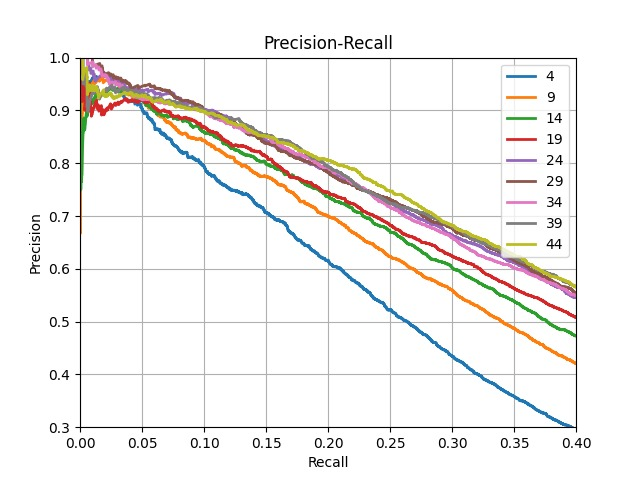
\includegraphics[width=4cm]{original.jpg}
        \caption{LSTM}
        \label{fig:lstm}
    \end{minipage}
    \begin{minipage}[t]{0.24\textwidth}
         \centering
         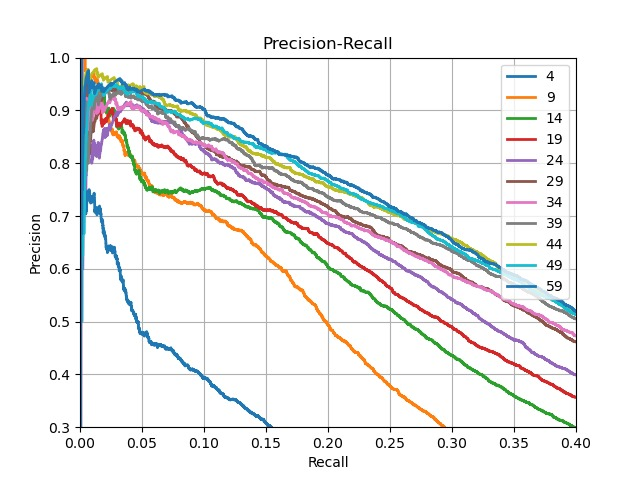
\includegraphics[width=4cm]{improved.jpg}
         \caption{UP-LSTM}
         \label{fig:up-lstm}
    \end{minipage}
    \begin{minipage}[t]{0.24\textwidth}
        \centering
        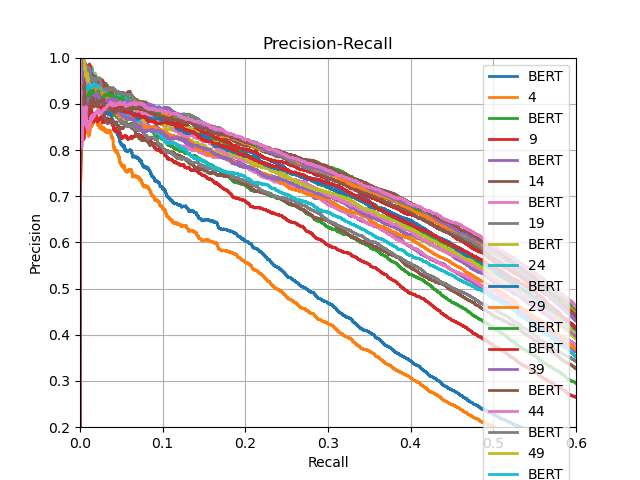
\includegraphics[width=4cm]{UP-BERT.png}
        \caption{UP-BERT}
        \label{fig:up-bert}
    \end{minipage}
\end{figure}

The UP-LSTM model offers a better balance between precision and recall, as can be seen from the PR curves. The UP-LSTM model appears to have a higher area under the PR curve (AUC), supporting this theory. A higher AUC suggests that the model performs better overall and that UP-LSTM is more skilled at identifying real associations without being tricked by false positives.It's also critical to see how the curves behave as they approach the recall axis' ends. The model may have reached the point where it can no longer identify true positives without producing false positives, as evidenced by the original LSTM curve's more severe tailing-off. However, the more gradual tailing off of the UP-LSTM points to a stronger capacity for generalization and resilience across thresholding levels.

\begin{table}[H]
    \caption{\textbf{Metrices on Dev and Test dataset(\%)}}
    \centering
    \begin{tabular}{ccccc}
        \toprule
        &\multicolumn{2}{c}{\textbf{\underline{Dev}}}
        &\multicolumn{2}{c}{\textbf{\underline{Test}}} \\
        Model&F1&AUC&F1&AUC \\
        \midrule
        LSTM\cite{yao2019docred}&44.37&39.58&50.14&49.31 \\
        LSTM (reappeared)&4.82&1.72&4.53&1.25 \\
        UP-LSTM&5.08&1.44&4.46&1.15 \\
        BERT\cite{zeng2020double}&54.16&50.13&53.25&49.56 \\
        UP-BERT&27.58&18.65&21.00&10.86 \\ 
        \bottomrule
    \end{tabular}
\end{table}

\begin{table}[H]
    \caption{\textbf{Methods Comparison by F1-Score(\%)}}
    \centering
    \begin{tabular}{ccccc}
        \toprule
        Model&F1&Model&F1\\
        \midrule
        UP-LSTM&4.46&UP-BERT&21.00 \\
        BiLSTM\cite{yao2019docred}&51.06&CNN\cite{yao2019docred}&42.33 \\
        SAIS-BERT\cite{xiao2021sais}&62.77&GAIN\cite{zeng2020double}&62.76\\
        SSAN\cite{xu2021entity}&58.16&DREEAM\cite{ma2023dreeam}&67.53 \\
        KD-Rb-l\cite{TanQingyu2022RD-A}&67.28&& \\
        \bottomrule
    \end{tabular}
\end{table}

Comparing F1-score (Table I) between original methods and updated methods on LSTM and BERT, it is clear that UP-BERT (27.58\%) illustrates approximately a 5 times increase than UP-LSTM (5.08\%) on dev dataset, and UP-LSTM shows higher F1-score than original LSTM (4.82\%) on dev dataset as well, but original LSTM (4.53\%) appears more effective than UP-LSTM (4.46\%) on test dataset. However, there is a big gap between LSTM and reappeared LSTM, UP-BERT and BERT, and UP-LSTM and LSTM. These may be related to insufficient training time, which need more experimentation to confirm. Furthermore, in Table II, comparing with other previous methods on DocRED dataset, BERT based methods (SAIS-62.77\%, SSAN-58.16\%) show better F1-score than other deep learning methods, such as BiLSTM (51.06\%), CNN (42.33\%) and GAIN (62.76\%). While, nowadays, DREEAM and KD-Rb-l as potential methods in the future show the highest score on the DocRED dataset: 67.53\% and 67.28\% respectively.

% (5) discuss the results of your evaluation, comparing the approaches and highlighting their strengths and weaknesses.

\section{Conclusion}

From this study, there are some exposed limitations of UP-LSTM, LSTM, and UP-BERT, which would be valuable to tackle in the future. Firstly, during the experiment of reappearing LSTM methods, the F1 score results have a big gap with results from a previous paper, as well as UP-LSTM and UP-BERT. For this issue, more experiments on reappearing need to be done in the future. Secondly, via comparison of different methods results, BERT methods illustrate more potential effort on NLP problems. Therefore, in the future, we could implement more in this direction. Finally, in our research, DREEAM\cite{ma2023dreeam} and KD-Rb-l\cite{TanQingyu2022RD-A} methods with tweaks to the attention mechanisms show outstanding effort on RE of DocRED dataset. Pursuing this direction could lead to further improvement.

\bibliography{references}
\bibliographystyle{unsrt}

\end{document}